\newpage
\section{Multi-Agent AI Module Pipeline}
\label{sec:multi-agent}

This section specifies the deployed AI module of H.E.R.A as an
operational pipeline. The goal is deterministic routing, bounded
latency, and explicit separation between language reasoning and
hardware side effects.

\subsection{Pipeline Definition}
\label{sec:mas-definition}

Let an incoming user message at step $t$ be
$u_t = (x_t, c_t, \tau_t)$, where:
\begin{itemize}
    \item $x_t$ is the text content,
    \item $c_t$ is the chat identifier,
    \item $\tau_t$ is the timestamp.
\end{itemize}

The AI module executes:
\begin{equation}
\label{eq:mas-pipeline}
    y_t = A_{\pi(C(x_t))}(u_t, s_t, h_t),
\end{equation}
where:
\begin{itemize}
    \item $C$ is the intent classifier,
    \item $\pi$ maps intent label to specialist agent,
    \item $A_k$ is specialist agent $k$,
    \item $s_t$ is current sensor snapshot from MQTT,
    \item $h_t$ is bounded dialogue history for chat continuity,
    \item $y_t$ is the final response sent to Telegram.
\end{itemize}

The classifier output set is fixed:
\begin{equation}
\label{eq:intent-set}
    \mathcal{I} = \{\texttt{device\_control},\; \texttt{sensor\_query},\;
    \texttt{anomaly\_query},\; \texttt{general}\}.
\end{equation}

Routing function:
\begin{equation}
\label{eq:routing-map}
\pi(i) =
\begin{cases}
\texttt{device\_control} & i = \texttt{device\_control}\\
\texttt{sensor\_analysis} & i = \texttt{sensor\_query}\\
\texttt{anomaly\_expert} & i = \texttt{anomaly\_query}\\
\texttt{chat} & \text{otherwise}
\end{cases}
\end{equation}

\subsection{Runtime Architecture}
\label{sec:mas-runtime}

The runtime is partitioned into four layers:
\begin{enumerate}
    \item \textbf{Adapter layer}: Telegram adapter transforms external
          events into internal \texttt{UserMessage} objects.
    \item \textbf{Orchestrator layer}: one router model classifies intent
          and dispatches to one specialist.
    \item \textbf{Specialist layer}: domain agents implement tool use,
          sensor interpretation, anomaly explanation, or general chat.
    \item \textbf{Service layer}: MQTT, LLM gateway, and tool registry
          provide side-effect and provider abstraction.
\end{enumerate}

\begin{figure}[H]
\centering
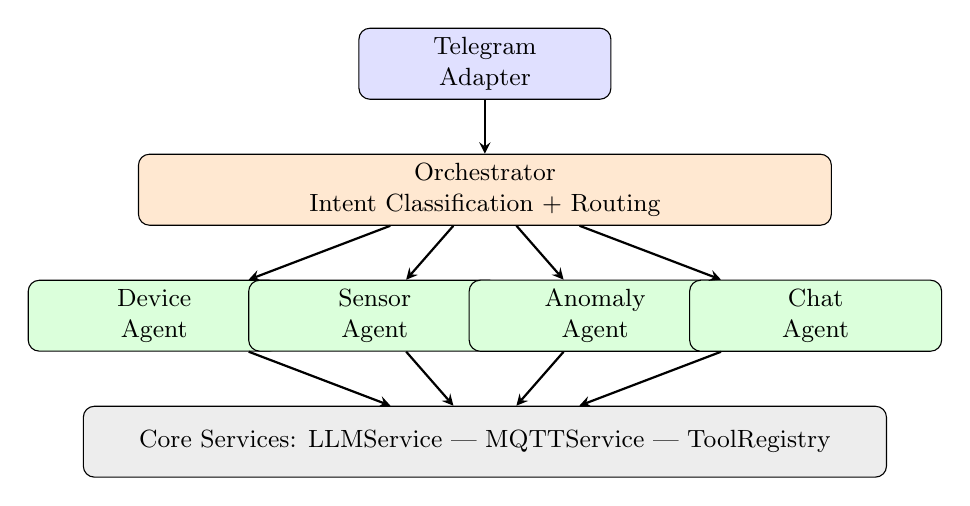
\begin{tikzpicture}[
    box/.style={draw, rounded corners, minimum width=3.2cm,
                minimum height=0.9cm, align=center, font=\small},
    arrow/.style={->, >=stealth, thick},
    every node/.style={font=\small}
]
\node[box, fill=blue!12] (tg) at (0,6) {Telegram\\Adapter};
\node[box, fill=orange!18, minimum width=8.8cm] (orch) at (0,4.4)
     {Orchestrator\\Intent Classification + Routing};

\node[box, fill=green!14] (dev) at (-4.2,2.8) {Device\\Agent};
\node[box, fill=green!14] (sen) at (-1.4,2.8) {Sensor\\Agent};
\node[box, fill=green!14] (ano) at (1.4,2.8) {Anomaly\\Agent};
\node[box, fill=green!14] (cha) at (4.2,2.8) {Chat\\Agent};

\node[box, fill=gray!14, minimum width=10.2cm] (core) at (0,1.2)
     {Core Services: LLMService | MQTTService | ToolRegistry};

\draw[arrow] (tg) -- (orch);
\foreach \a in {dev,sen,ano,cha} {
    \draw[arrow] (orch) -- (\a);
    \draw[arrow] (\a) -- (core);
}
\end{tikzpicture}
\caption{Final multi-agent runtime topology.}
\label{fig:mas-arch}
\end{figure}

\subsection{Agent Contract and Model Assignment}
\label{sec:mas-agent-spec}

All specialists implement the same contract:
\begin{equation}
\label{eq:agent-interface}
    (u_t, \texttt{context}) \mapsto
    (\texttt{text},\; \texttt{tools\_used},\; \texttt{metadata}).
\end{equation}

This uniform interface allows the orchestrator to swap specialists
without adapter changes.

\begin{table}[H]
\centering
\caption{Agent roles and model control keys in \texttt{.env}.}
\label{tab:agent-model-map}
\renewcommand{\arraystretch}{1.25}
\begin{tabularx}{\textwidth}{l l X}
    \toprule
    \textbf{Module} & \textbf{Role} & \textbf{Model Key(s)} \\
    \midrule
    Orchestrator & Intent routing
      & \texttt{ORCHESTRATOR\_MODEL\_OLLAMA},
        \texttt{ORCHESTRATOR\_MODEL\_OPENROUTER} \\
    Device Agent & LED / actuator command execution
      & \texttt{DEVICE\_AGENT\_MODEL\_OLLAMA},
        \texttt{DEVICE\_AGENT\_MODEL\_OPENROUTER} \\
    Sensor Agent & Sensor-state interpretation
      & \texttt{SENSOR\_AGENT\_MODEL\_OLLAMA},
        \texttt{SENSOR\_AGENT\_MODEL\_OPENROUTER} \\
    Anomaly Agent & Anomaly severity explanation
      & \texttt{ANOMALY\_AGENT\_MODEL\_OLLAMA},
        \texttt{ANOMALY\_AGENT\_MODEL\_OPENROUTER} \\
    Chat Agent & General conversation fallback
      & \texttt{CHAT\_AGENT\_MODEL\_OLLAMA},
        \texttt{CHAT\_AGENT\_MODEL\_OPENROUTER} \\
    \bottomrule
\end{tabularx}
\end{table}

\subsection{Tool-Execution Semantics}
\label{sec:mas-tool-semantics}

For a tool-call sequence of length $n \leq N_{\max}$, where
$N_{\max}=\texttt{MAX\_TOOL\_ITERATIONS}$:
\begin{equation}
\label{eq:tool-loop}
    m_{k+1} = \mathcal{L}(m_k, r_k), \quad
    r_k = T(f_k, a_k), \quad k = 0,1,\dots,n-1,
\end{equation}
with:
\begin{itemize}
    \item $\mathcal{L}$: selected LLM backend,
    \item $f_k$: tool function name,
    \item $a_k$: function arguments,
    \item $T$: registry executor that publishes MQTT RPC and updates
          shared state.
\end{itemize}

The command set for device control is finite:
\begin{equation}
\label{eq:tool-set}
\mathcal{T}_{\text{device}} =
\{\texttt{turn\_on\_led},\texttt{turn\_off\_led},
\texttt{turn\_on\_neo\_led},\texttt{turn\_off\_neo\_led},
\texttt{turn\_on\_all\_lights},\texttt{turn\_off\_all\_lights}\}.
\end{equation}

Sensor module additionally exposes:
\begin{equation}
\label{eq:sensor-tool}
\mathcal{T}_{\text{sensor}} = \{\texttt{get\_sensor\_status}\}.
\end{equation}

\subsection{Per-Chat Memory Rule}
\label{sec:mas-history}

History is tracked by chat ID:
\begin{equation}
\label{eq:history-window}
    h_t(c) = \operatorname{tail}_{M}(h_{t-1}(c) \cup \{x_t, y_t\}),
\end{equation}
where $M=\texttt{MAX\_HISTORY}$.

If any tool is executed in the current turn, history is reset:
\begin{equation}
\label{eq:history-reset}
    \texttt{tools\_used} \neq \emptyset \Rightarrow h_t(c)=\emptyset.
\end{equation}

This avoids carrying stale actuator/tool context into unrelated future
turns.

\subsection{Configuration Surface in \texttt{.env}}
\label{sec:mas-config}

The finalized module is controlled through environment keys, grouped
as follows:
\begin{itemize}
    \item \textbf{Provider and model routing}: \texttt{LLM\_PROVIDER},
          default model keys, orchestrator model keys, specialist model
          keys.
    \item \textbf{MQTT connectivity and topics}: broker host/port and
          topic namespace keys.
    \item \textbf{AI thresholds}: normal temperature/humidity ranges and
          anomaly score thresholds.
    \item \textbf{Pipeline limits}: tool-call cap and history window size.
    \item \textbf{Adapter runtime}: Telegram timeout values.
    \item \textbf{Simulator control}: telemetry interval and physical
          clamp ranges for generated signals.
\end{itemize}

With this layout, changing model orchestration or runtime behavior
requires only \texttt{.env} edits; no source-code modification is
needed.

\subsection{Execution Path}
\label{sec:mas-sequence}

\begin{figure}[H]
\centering
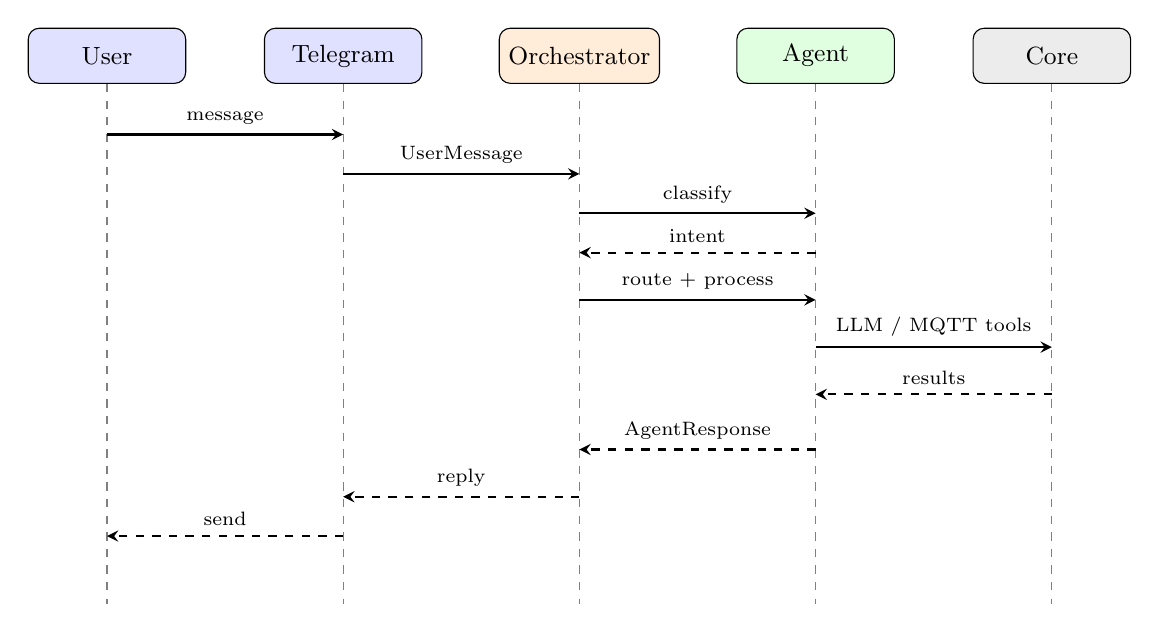
\begin{tikzpicture}[
    font=\small,
    box/.style={draw, rounded corners, fill=#1, minimum width=2cm,
                minimum height=0.7cm, align=center},
    arr/.style={->, >=stealth, thick},
]
\node[box=blue!12]   (user) at (0,0) {User};
\node[box=blue!12]   (tg)   at (3,0) {Telegram};
\node[box=orange!15] (orch) at (6,0) {Orchestrator};
\node[box=green!12]  (agt)  at (9,0) {Agent};
\node[box=gray!15]   (srv)  at (12,0) {Core};

\foreach \n in {user,tg,orch,agt,srv} {
    \draw[dashed, gray] (\n.south) -- ++(0,-6.6);
}

\draw[arr] (0,-1)   -- node[above,font=\scriptsize]{message} (3,-1);
\draw[arr] (3,-1.5) -- node[above,font=\scriptsize]{UserMessage} (6,-1.5);
\draw[arr] (6,-2.0) -- node[above,font=\scriptsize]{classify} (9,-2.0);
\draw[arr,dashed] (9,-2.5) -- node[above,font=\scriptsize]{intent} (6,-2.5);
\draw[arr] (6,-3.1) -- node[above,font=\scriptsize]{route + process} (9,-3.1);
\draw[arr] (9,-3.7) -- node[above,font=\scriptsize]{LLM / MQTT tools} (12,-3.7);
\draw[arr,dashed] (12,-4.3) -- node[above,font=\scriptsize]{results} (9,-4.3);
\draw[arr,dashed] (9,-5.0) -- node[above,font=\scriptsize]{AgentResponse} (6,-5.0);
\draw[arr,dashed] (6,-5.6) -- node[above,font=\scriptsize]{reply} (3,-5.6);
\draw[arr,dashed] (3,-6.1) -- node[above,font=\scriptsize]{send} (0,-6.1);
\end{tikzpicture}
\caption{Operational request path of the AI module.}
\label{fig:sequence}
\end{figure}

\subsection{Summary}
\label{sec:mas-summary}

The AI module is fixed as an orchestrator-specialist pipeline with:
\begin{itemize}
    \item explicit intent-to-agent mapping,
    \item bounded tool loop and bounded chat memory,
    \item MQTT-mediated side effects through a centralized registry,
    \item fully externalized model/runtime configuration in
          \texttt{backend/HERA/.env}.
\end{itemize}

This definition is the implementation baseline used by the simulator
and Telegram runtime in the current thesis build.
